% Welcome! This is the unofficial University of Udine beamer template.

% See README.md for more informations about this template.

% This style has been developed following the "Manuale di Stile"
% (Style Manual) of the University of Udine. You can find the
% manual here: https://www.uniud.it/it/ateneo-uniud/ateneo-uniud/identita-visiva/manuali-immagine-stile/manuale-stile

% Note: for some reason, the RGB values specified in the manual
% do NOT render correctly in Beamer, so they have been redefined
% for this document using the high level chromo-optic deep neural
% quantistic technology offered by Microsoft Paint's color picker.

% We defined four theme colors: UniBrown, UniBlue, UniGold
% and UniOrange. For example, to write some uniud-brownish
% text, just use: \textcolor{UniBrown}{Hello!}

% Note that [usenames,dvipsnames] is MANDATORY due to compatibility
% issues between tikz and xcolor packages.

\documentclass[usenames,dvipsnames]{beamer}
\usepackage[utf8]{inputenc}
\usepackage{verbatim}
\usetheme{uniud}

% cleverref {{{
\usepackage[capitalize,nameinlink]{cleveref} % from https://tex.stackexchange.com/questions/187388/amsthm-with-shared-counters-messes-up-autoref-references
% }}}

\usepackage{graphicx}

%%% Bibliography {{{
% \usepackage[style=authoryear,backend=biber]{biblatex}
\usepackage[style=alphabetic,backend=biber]{biblatex}
\addbibresource{bibliography.bib}

% Author names in publication list are consistent
% i.e. name1 surname1, name2 surname2
% See https://tex.stackexchange.com/questions/106914/biblatex-does-not-reverse-the-first-and-last-names-of-the-second-author
\DeclareNameAlias{author}{first-last}
% }}}

%%% Suppress biblatex annoying warning {{{
\usepackage{silence}
\WarningFilter{biblatex}{Patching footnotes failed}
% }}}

%%% Some useful commands {{{
% pdf-friendly newline in links
\newcommand{\pdfnewline}{\texorpdfstring{\newline}{ }}
% Fill the vertical space in a slide (to put text at the bottom)
\newcommand{\framefill}{\vskip0pt plus 1filll}
% }}}

% \title[University of Udine Unofficial Beamer Theme]{Report: A formal approach for run-time verification of web applications using scope-extended LTL}
\title{Run-time verification of web applications}
\date{March 21st, 2025}
\author[Roberto Tonino]{
  Roberto Tonino
  \pdfnewline
  \texttt{tonino.roberto@spes.uniud.it}
}
\institute{\tiny Department of Mathematics, Computer Science and Physics, University of Udine}

% glossary {{{
\usepackage[acronym,automake]{glossaries}
\makeglossaries

% \newglossaryentry{WAUT}
% {
%     name=WAUT,
%     description={Web Application Under Test}
% }
\newacronym{waut}{WAUT}{Web Application Under Test}
\newacronym{spa}{SPA}{Single Page Application}
\newacronym{ssg}{SSG}{Static Site Generator}
% }}}

\usepackage{ifthen}

\newcommand{\tuple}[1]{\mbox{$\langle$#1$\rangle$}}
% \newcommand{\reqmulti}[1]{\mbox{$\langle r_{#1}$,$l_{#1}$,$t_{#1}\rangle$}}
\newcommand{\reqmulti}[1][]{
  \ifthenelse{\equal{#1}{}} {\mbox{$\langle r$,$l$,$t\rangle$}}
  {\mbox{$\langle r_{#1}$,$l_{#1}$,$t_{#1}\rangle$}}
}

\newcommand{\res}[1][]{
  \ifthenelse{\equal{#1}{}}{\mbox{$\langle u$, $c$, $I$, $L$, $V\rangle$}}
  {\mbox{$\langle u_{#1}$, $c_{#1}$, $I_{#1}$, $L_{#1}$, $V_{#1}\rangle$}}
}
\newcommand{\resmulti}[1][]{
  \ifthenelse{\equal{#1}{}}{\mbox{$\langle u$, $c$, $I$, $F$, $L$, $V\rangle$}}
  {\mbox{$\langle u_{#1}$, $c_{#1}$, $I_{#1}$, $F_{#1}$, $L_{#1}$, $V_{#1}\rangle$}}
}

\usepackage{amsthm}

% \theoremstyle{plain} % default
% \newtheorem{lem}[thm]{Lemma}
% \newtheorem{proposition}[thm]{Proposition}
% \newtheorem*{cor}{Corollary}

\theoremstyle{definition}
% \newtheorem{definition}{Definition}
\newtheorem{procedure}{Procedure}

% \theoremstyle{remark}
% \newtheorem{rmrk}{Remark}[section]
% \newtheorem{note}{Note}[section]

\usepackage[capitalize,nameinlink]{cleveref} % from https://tex.stackexchange.com/questions/187388/amsthm-with-shared-counters-messes-up-autoref-references
% Customize cref names
% Generated by Claude
% \crefname{rmrk}{Remark}{Remarks}
% \crefname{lem}{Lemma}{Lemmas}
\crefname{procedure}{Procedure}{Procedures}


\begin{document}

\begin{frame}
\titlepage
\end{frame}

% \begin{frame}{Outline}
% \tableofcontents
% \end{frame}

% \section{Before you start}
% \begin{frame}{Overleaf users}

% \begin{alertblock}{Warning}
% You can ignore this slide if you're \textbf{not} working with Overleaf.
% \end{alertblock}

% \vskip 0.5cm

% Overleaf, Beamer and Biber do not always get along well together. For this reason, if you make a mistake while writing this presentation, in the drop-down error message you'll \textbf{always} get Biber-related error messages.

% \vskip 0.5cm

% Luckily, you just have to click on ``\texttt{go to first error/warning}'' and the UI will scroll to the line containing your mistake.

% \end{frame}

\section{Overview}
\begin{frame}{Overview}

  \begin{itemize}
    \item Paper from 2013
    \item Tool for automatic verification of web applications
    \item Empirical results
  \end{itemize}
\end{frame}

\begin{frame}{Overview}
  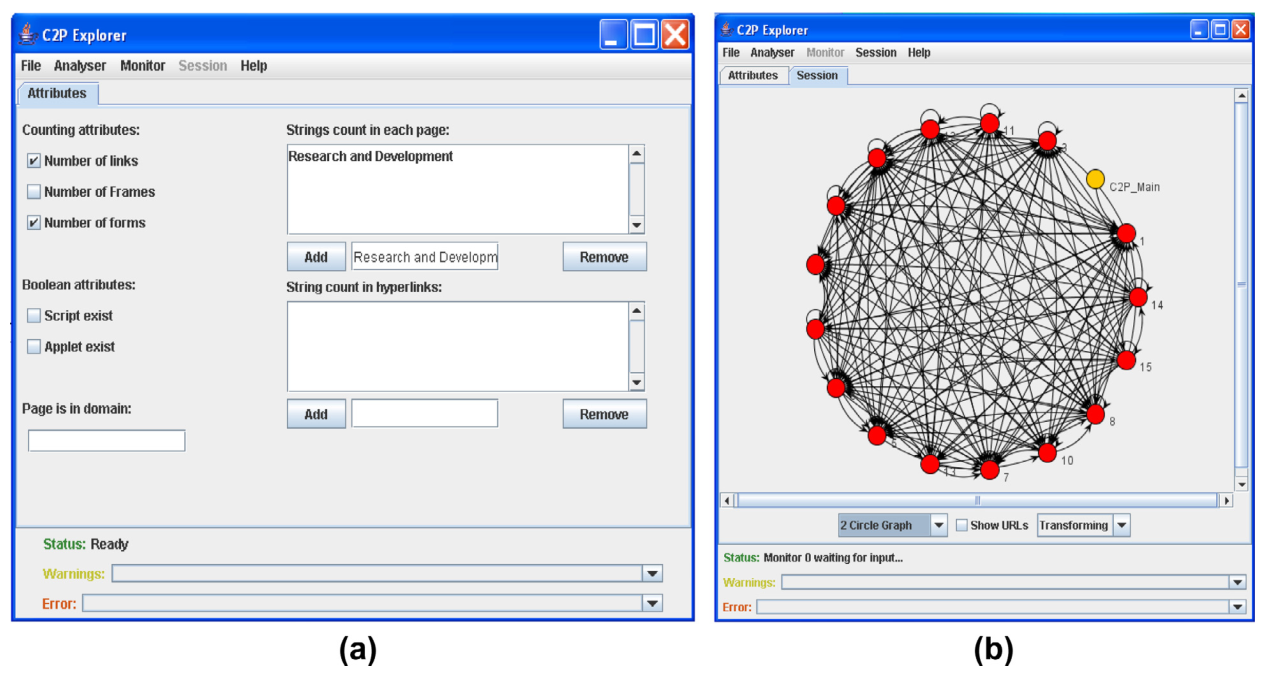
\includegraphics[width=\textwidth]{../img/screenshot_tool.png}
\end{frame}

\section{How?}
\begin{frame}{How?}
  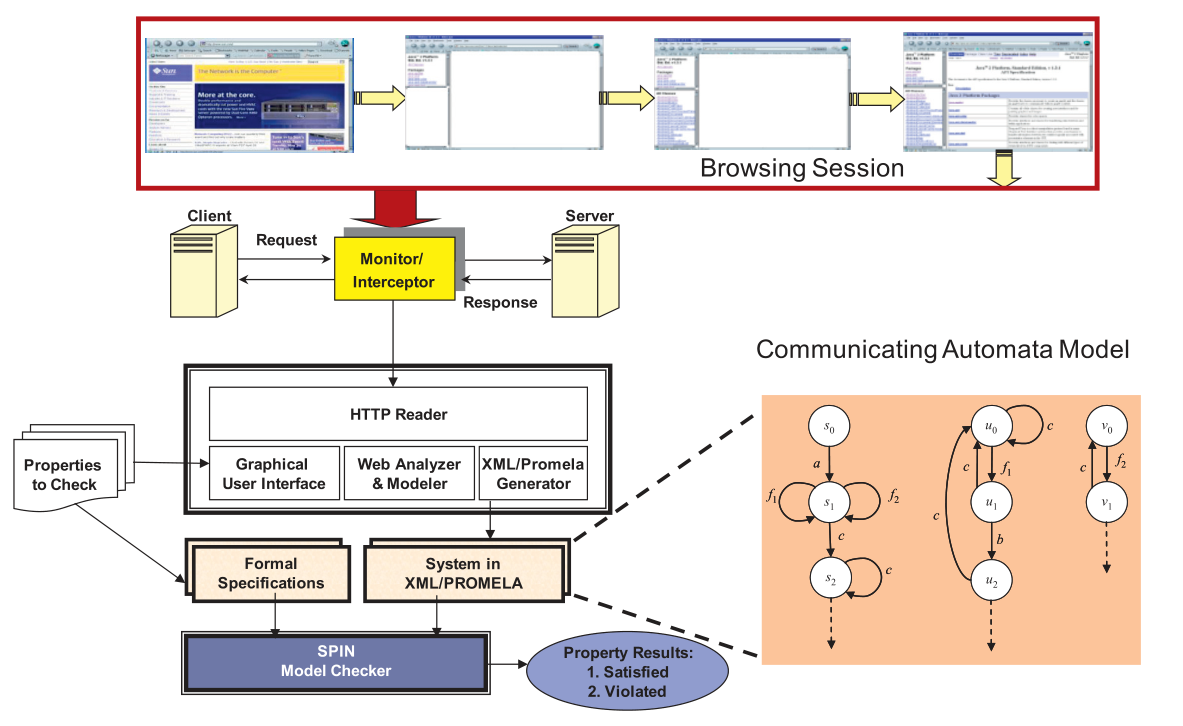
\includegraphics[width=\textwidth]{../img/general_architecture.png}
\end{frame}

\begin{frame}{Some definitions first}
  \begin{itemize}
    \item \textit{\gls{waut}}: the web application taken in consideration in a particular definition, discussion, etc...
    \item \textit{request}: string $l$ that represents a web request performed by a \gls{waut}
    \item \textit{response}: tuple \res which represents the response that the web server sent to the \gls{waut}
      \begin{itemize}
        \item $u = l$
        \item $c$ represents the status code of the response \cite{Fielding2022}
        \item $I =$ ``target'' attribute of the forms contained in the response
        \item $L =$ URLs of the links contained in the response
        \item $V =$\ <$v_1,\dots,v_k$> vector where $v_i$ is the valuation of the page attribute $i$
      \end{itemize}
  \end{itemize}
\end{frame}

\begin{frame}{Some definitions first}
  \begin{itemize}
    \item \textit{browsing session}: denoted $RRS$, it is a recorded sequence of request-response exchanges that a user performs when visiting a \gls{waut}
    \item \textit{local browsing session}: denoted $RRS$ as well, it is a recorded sequence of request-response exchanges that a user performs in a single browser window or frame
  \end{itemize}
\end{frame}

\framecard{Communicating automata model}

\section{Single-display automaton}
\begin{frame}[t,allowframebreaks]{Single-display automaton}
  Convert a browsing session of a single-display application into an automaton.

  \begin{enumerate}
    \item the inactive state $s_0 = \res[0]$ is defined;
    \item the set of states is defined by the set of \emph{responses}, a response being \res[i]
      % \begin{enumerate}
      %   \item when only the links in two responses are different, the responses are mapped to the same state. The authors provide a proof that this compression does not alter the recorded behaviour of the \gls{waut};
      % \end{enumerate}
    \item the alphabet is built from the union of the requests ($Req$), the URIs associated with links in the observed responses ($\Gamma$), and the actions that correspond to the unexplored forms in the observed responses $\Delta$. $\Sigma=Req\cup\Gamma\cup\Delta$;
    \item there is a transition $(s_i,l_{i+1},s_{i+1})$ from state $s_i$ to state $s_{i+1}$ if there is a \textbf{link} or a \textbf{form action} that goes from the page represented by $s_i$ to the page represented by $s_{i+1}$;
    \item requests corresponding to explored forms or links define a transition that goes from the state where the request occurs to the state mapped to the response;
    \item for each unexplored link $l \in L_i$ or form $a \in I_i$, the automaton has a transition from the state representing the page \res[i] to a so-called \textit{trap} state $t \in T$.
  \end{enumerate}
\end{frame}

\begin{frame}{Deduced links}
  \begin{itemize}
    \item from the construction of a single-display automaton, it is possible to derive \textbf{deduced} links
    \item i.e.\ links that are not visited during the browsing session, but present in at least one of the responses
  \end{itemize}
\end{frame}

\begin{frame}{Example of single-display automaton}
  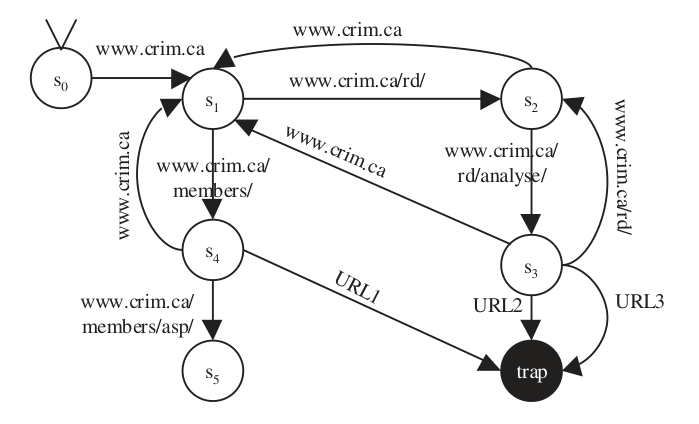
\includegraphics[width=\textwidth]{../img/session_automaton_example.png}
\end{frame}

\section{Multi-display automaton}
\begin{frame}{Multi-display automaton}
  From single-display to multi-display:
  \begin{itemize}
    \item \textit{response:} \resmulti with $F$ being a set of frames in the page. The target $t$ is defined; if no target is present $t = \varepsilon$. Additional changes are:
      \begin{itemize}
        \item \tuple{$i$, $t$} $\in L$
        \item \tuple{$a$, $t$} $\in I$
        \item \tuple{$f$,$b$} $\in F$
      \end{itemize}
    \item the requests are now made of the link as before, with the addition of the referer $r$ (link from which the request started) and the target $t$. They are denoted as \reqmulti
  \end{itemize}
\end{frame}

\begin{frame}{Communicating automata model}
  Convert a browsing session of a multi-display application into a communicating automata model.

  \begin{enumerate}
    \item a browsing session is split into a local browsing session $(RRS_1,\dots,RRS_k)$, one for each window and frame;
    \item convert each local browsing session into an automaton;
      \begin{enumerate}
        \item convert a $RRS$ to a single-display automaton;
        \item the alphabet $\Sigma_i$ is extended with the source pages of the frames (src attribute), $\Sigma_i := \Sigma_i\cup\Phi_i$;
        \item the case in which the user clicks on a link or submits a form while a frame is loading is handled by adding a transition from each state of the local automaton to the response state;
        \item each unexplored link \reqmulti[i]$\in\Gamma_i$ is mapped to a loop in the state it targets (self-loop);
      \end{enumerate}
    \item create the communicating automata via the \textit{parallel composition operator}, denoted $A_1\mid\mid A_2$. The compositions of multiple automata is denoted $A_1\mid\mid\dots\mid\mid A_k$
  \end{enumerate}
\end{frame}

\begin{frame}{Extending the automata model}
  \begin{itemize}
    \item there is the need to characterize states of the automata
    \item because the browser automatically triggers frame requests upon loading the page that contains them
    \item extension happens via addition of a \textit{context variable}
  \end{itemize}
\end{frame}

\begin{frame}
  \frametitle{Extending the automata model}
  \framesubtitle{Single-display automaton}

  \begin{enumerate}
    \item the set of states $S_i$, alphabet $\Sigma_i$ and initial state $s_{0i}$ are unchanged;
    \item $x_i$ is the context variable of $Q_i$, $x_{0i}$ is the context variable's initial state;
    \item for each transition $(s,a,s')\in T_i$, $s,s'\in S_i$, $a\in\Sigma_i$:
      \begin{enumerate}
        \item if $s=s'$ and $a\in\Sigma^d_i$, then $(s,a,x_i := x_i - 1,s)$ is a transition in $Q_i$, where $x_i := x_i - 1$ is the update of the transition; or
        \item $(s,a,x_i := |init(s')\cap \Sigma^d_i|,s')$ is a transition in $Q_i$, where $x_i := |init(s')\cap\Sigma^d_i|$ is the update of the transition.
        \item ($\Sigma^d_i$ is the set of those transitions who cause the automaton to pass through a transient state, called ``designated set of transitions'')
      \end{enumerate}
  \end{enumerate}
\end{frame}


\begin{frame}
  \frametitle{Extending the automata model}
  \framesubtitle{Multi-display automaton}

  \begin{enumerate}
    \item build the single-display automata;
    \item extend each automaton;
    \item the set of designated events $\Sigma^d_i$ is the \textbf{set of frames of the browsing session};
    \item $x_i$ is initially set to 0;
    \item at each state $s_i$, $x_i$ is the number of browser triggered events enabled in $s_i$;
    \item each automaton is unfolded (transformed to its equivalent non-extended version);
    \item the unfolded automata are composed using the composition operator.
  \end{enumerate}
\end{frame}

\framecard{Property specification}

\begin{frame}{Property specification}
  \begin{itemize}
    \item LTL is used
    \item authors introduce 2 new operators that allow to specify properties over a subset of the state
    \item $\mathcal{\Im}$-scope operator over \textbf{propositional logic expressions}
    \item \textbf{\texttt{In}} operator over \textbf{logical formulas}
  \end{itemize}
\end{frame}

\begin{frame}{Example}
  \begin{example}
    \begin{gather}
      G(((\neg Home\land\neg Shopping) \rightarrow (Promotions = 0)) \land \nonumber \\
      ((Home\land Shopping) \rightarrow (Promotions \leq 2))) \nonumber
    \end{gather}
  \end{example}

  simplifies to

  \begin{example}
    \label{example:in-operator-simple}
    $$
    G(((Promotions \leq 2)\ \textbf{\texttt{In}}\ (Home\lor Shopping))\lor(Promotions=0))
    $$
  \end{example}
\end{frame}

\section{Implementation and empirical evaluation}
\framecard{Implementation and empirical evaluation}

\begin{frame}{Implementation and empirical evaluation}
  \begin{itemize}
    \item the tool can
      \begin{itemize}
        \item record a browsing session
        \item build an internal representation of the session
        \item evaluate a set of properties against the internal representation
        \item visualize the communicating automata
      \end{itemize}
    \item the set of properties are categorized as
      \begin{itemize}
        \item non-functional/general
        \item functional/specific
      \end{itemize}
  \end{itemize}
\end{frame}

\begin{frame}{Properties}
  \begin{itemize}
    \item Non-functional:
      \begin{enumerate}
        \item Broken links and deadlocks are absent.
        \item Number of links in each display (single or multi) should not exceed a certain threshold (depends on size of application).
        \item Number of images in each display (single or multi) should not exceed a certain threshold (depends on size of application).
        \item Number of links in each display (single or multi) is balanced.
        \item Combinations of certain words/objects are absent.
      \end{enumerate}
  \end{itemize}
\end{frame}

\begin{frame}{Properties}
  \begin{itemize}
    \item Functional 
      \begin{enumerate}
        \item Home page is reachable from every other page.
        \item Page X is reachable from page Y without going through a cer- tain page Z.
        \item Secure pages are not reachable without authentication process.
        \item In e-commerce applications, promotions of certain products are only present either on the Home page or on Shopping pages and, for each page, the number of promotions does not exceed two.
        \item Privacy policy page in e-commerce applications is reachable from every page.
      \end{enumerate}
  \end{itemize}
\end{frame}

\begin{frame}{Results}
  \begin{itemize}
    \item most of the properties were violated
    \item small and large \gls{waut} have \textbf{less} violation compared to medium-sized ones
  \end{itemize}
\end{frame}

\begin{frame}{Counterexample}
  An example of a specification where the authors found a counterexample:

  \begin{example}
    \begin{math}
      G((montreal\land fire\land underg)\lor((montreal\land fire)\lor((montreal\land underg)\lor((underg\land fire)\lor montreal\lor underg\lor fire))))
    \end{math}
  \end{example}
\end{frame}

\begin{frame}{Counterexample}
  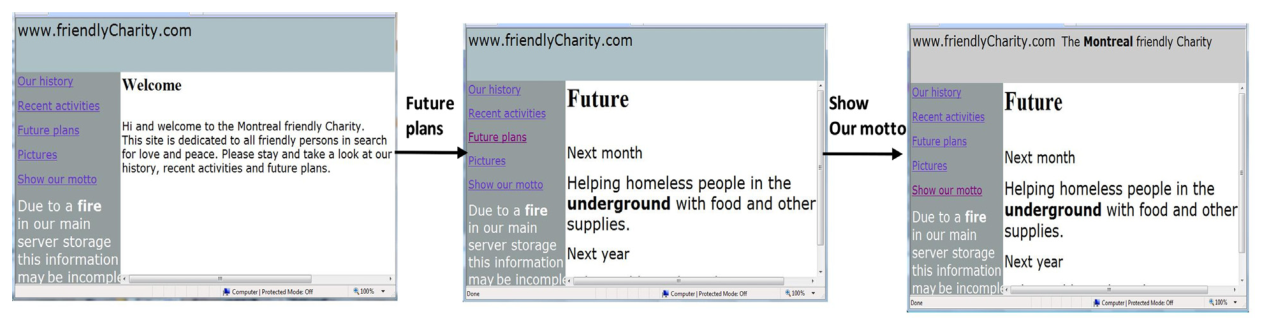
\includegraphics[width=\textwidth]{../img/counterexample.png}
\end{frame}

\section{Conclusions}
\framecard{Conclusions}

\begin{frame}{Conclusions}
  \begin{itemize}
    \item using multiple frames is not common practice in web app development
    \item nowadays applications are client-side rendered (via JavaScript) starting from JSON instead of HTML 
    \item the approach presented might be more useful for websites, which use more of a mixed approach compared to web applications
  \end{itemize}
\end{frame}

\section{Bibliography}
\framecard{Bibliography}

\begin{frame}[t,allowframebreaks]{Bibliography}
  \nocite{*} % will display the non-cited publications as well. Useful for a publication list.
  \printbibliography
\end{frame}

\end{document}

% vi: fdm=marker
